% no notes
\documentclass{beamer}
% notes and slides
%\documentclass[notes]{beamer}
% notes only
% \documentclass[notes=only]{beamer}
\usepackage{graphicx} % Allows including images
\usepackage{booktabs} % Allows the use of \toprule, \midrule and \bottomrule in tables
\usepackage{multirow}
\usepackage{multimedia}
\usepackage{tikz}
\usepackage{circuitikz}
\usepackage{url}
\usepackage{pgfplots}
\usepackage{pgfplots}
%\DeclareUnicodeCharacter{2212}{−}
\usepgfplotslibrary{groupplots,dateplot}
\usetikzlibrary{patterns,shapes.arrows}
\pgfplotsset{compat=newest}
\usepackage{standalone}
\usepackage{adjustbox}
\usepackage{lmodern}
\usepackage{pgfplots}
\usepackage{amsmath}
\usepackage{amsthm}
\usepackage{multimedia}
\usepackage{standalone}
\usepackage{csquotes}

% from https://tex.stackexchange.com/questions/83882/how-to-highlight-python-syntax-in-latex-listings-lstinputlistings-command
% Default fixed font does not support bold face
\DeclareFixedFont{\ttb}{T1}{txtt}{bx}{n}{12} % for bold
\DeclareFixedFont{\ttm}{T1}{txtt}{m}{n}{12}  % for normal

% Custom colors
\usepackage{color}
\definecolor{deepblue}{rgb}{0,0,0.5}
\definecolor{deepred}{rgb}{0.6,0,0}
\definecolor{deepgreen}{rgb}{0,0.5,0}

\usepackage{listings}

% Python style for highlighting
\newcommand\pythonstyle{\lstset{
language=Python,
basicstyle=\ttm,
morekeywords={self},              % Add keywords here
keywordstyle=\ttb\color{deepblue},
emph={MyClass,__init__},          % Custom highlighting
emphstyle=\ttb\color{deepred},    % Custom highlighting style
stringstyle=\color{deepgreen},
frame=tb,                         % Any extra options here
showstringspaces=false
}}


% Python environment
\lstnewenvironment{python}[1][]
{
\pythonstyle
\lstset{#1}
}
{}

% Python for external files
\newcommand\pythonexternal[2][]{{
\pythonstyle
\lstinputlisting[#1]{#2}}}

% Python for inline
\newcommand\pythoninline[1]{{\pythonstyle\lstinline!#1!}}


\PassOptionsToPackage{american}{babel} % change this to your language(s), main language last
% Spanish languages need extra options in order to work with this template
% \PassOptionsToPackage{spanish,es-lcroman}{babel}
\usepackage{babel}

\PassOptionsToPackage{%
  backend=biber,bibencoding=utf8, %instead of bibtex
  %backend=bibtex8,bibencoding=ascii,%
  language=auto,%
  style=numeric-comp,%
  %style=authoryear-comp, % Author 1999, 2010
  %bibstyle=authoryear,dashed=false, % dashed: substitute rep. author with ---
  style=alphabetic,
  sorting=nyt, % name, year, title
  maxbibnames=10, % default: 3, et al.
  %backref=true,%
  %natbib=true % natbib compatibility mode (\citep and \citet still work)
}{biblatex}
\usepackage{biblatex}

\addbibresource{bib.bib}

\usetheme{metropolis}           % Use metropolis theme
\setbeamertemplate{caption}[default]
\title{Explaining neural networks}
\date{10.03.24}
\institute{High-Performance Computing and Analytics Lab}
\author{Moritz Wolter}

\titlegraphic{
\includegraphics[width=2.00cm]{UNI_Bonn_Logo_Standard_RZ.pdf}}
\begin{document}
    \maketitle

    \begin{frame}
    \frametitle{Overview} 
    \tableofcontents
    \end{frame}

    \begin{frame}{Motivation}
      \begin{itemize}
        \item Neural networks are potent black-box methods.
        \item Some very deep convolutional neural networks have hundreds of layers and use up to 600mb of disk storage.
        \item Let's do what we can to open the box!!
      \end{itemize}
    \end{frame}

    \section{Linear classifiers}
    \begin{frame}{Definition of a linear classifier}
      Linear classifiers consist of a dense layer without an activation,
      \begin{align}
        \mathbf{o} = \mathbf{A}\mathbf{x} + \mathbf{b}.
      \end{align}
      With $\mathbf{A} \in \mathbb{R}^{m,n}, \mathbf{x} \in \mathbb{R}^{n}$ and $\mathbf{b} \in \mathbb{R}^{n}$.
      Linear only works on simple problems that are linearly separable.
    \end{frame}

    \begin{frame}{Binary MNIST}
      \begin{figure}
        \includestandalone[width=0.49\linewidth]{./figures/mnist_mean_6}
        \includestandalone[width=0.49\linewidth]{./figures/mnist_mean_9}
      \end{figure}
    \end{frame}

    \begin{frame}{Cross-Entropy}
      Recall the definition of the cross entropy
      \begin{align}
        C_{\text{ce}}(\mathbf{y}, \mathbf{o}) = -\sum_k^{n_o} ( \mathbf{y}_k  \ln \mathbf{o}_k) 
                                   + (\mathbf{1} - \mathbf{y}_k)
                                      \ln(\mathbf{1} - \mathbf{o}_k).
       \end{align}
       With $\mathbf{y},\mathbf{o} \in \mathbb{R}^{n_o}$ defined as vectors of length $n_o$.
    \end{frame}

    \begin{frame}{Cross-Entropy}
      To understand what is going on lets consider the two cases $y_k = 0$ and $y_k = 1$.
      \begin{figure}
        \includestandalone[width=0.45\linewidth]{./figures/ce_label_0}
        \includestandalone[width=0.45\linewidth]{./figures/ce_label_1}
      \end{figure}
      Cross-entropy pushes the output towards the label.
    \end{frame}

    \subsection{Interpretation by examination}
    \begin{frame}{Interpretation by examination}
      \begin{figure}
        \includestandalone[width=0.49\linewidth]{./figures/mnist_linear_6}
        \includestandalone[width=0.49\linewidth]{./figures/mnist_linear_9}
      \end{figure}
      If linear is possible linear is great!!
    \end{frame}

    \subsection{Case Study: Deepfake detection}

    \begin{frame}{What deep-fakes are}
      Generative models can generate images. Consider the samples below:
      \begin{figure}
      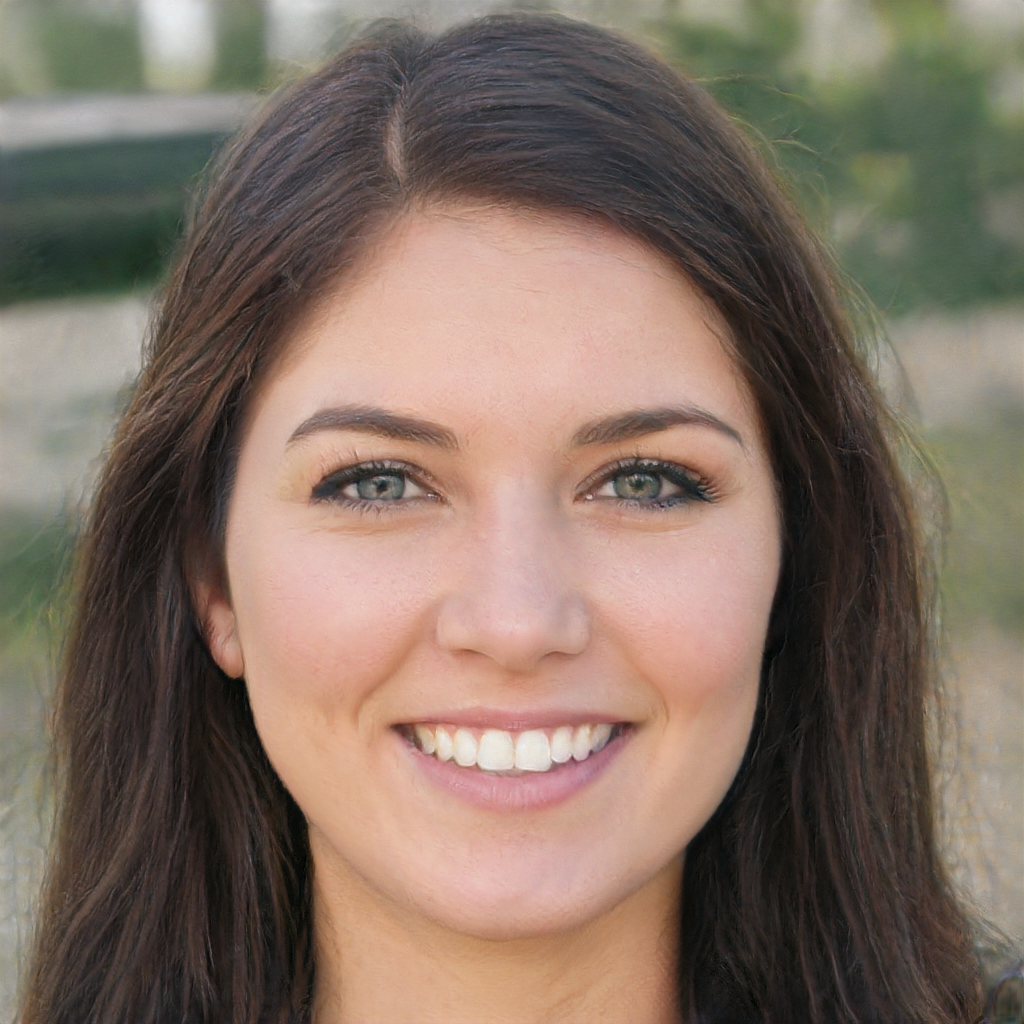
\includegraphics[width=0.32\linewidth]{./figures/style_gan_ffhq_example300.png}
      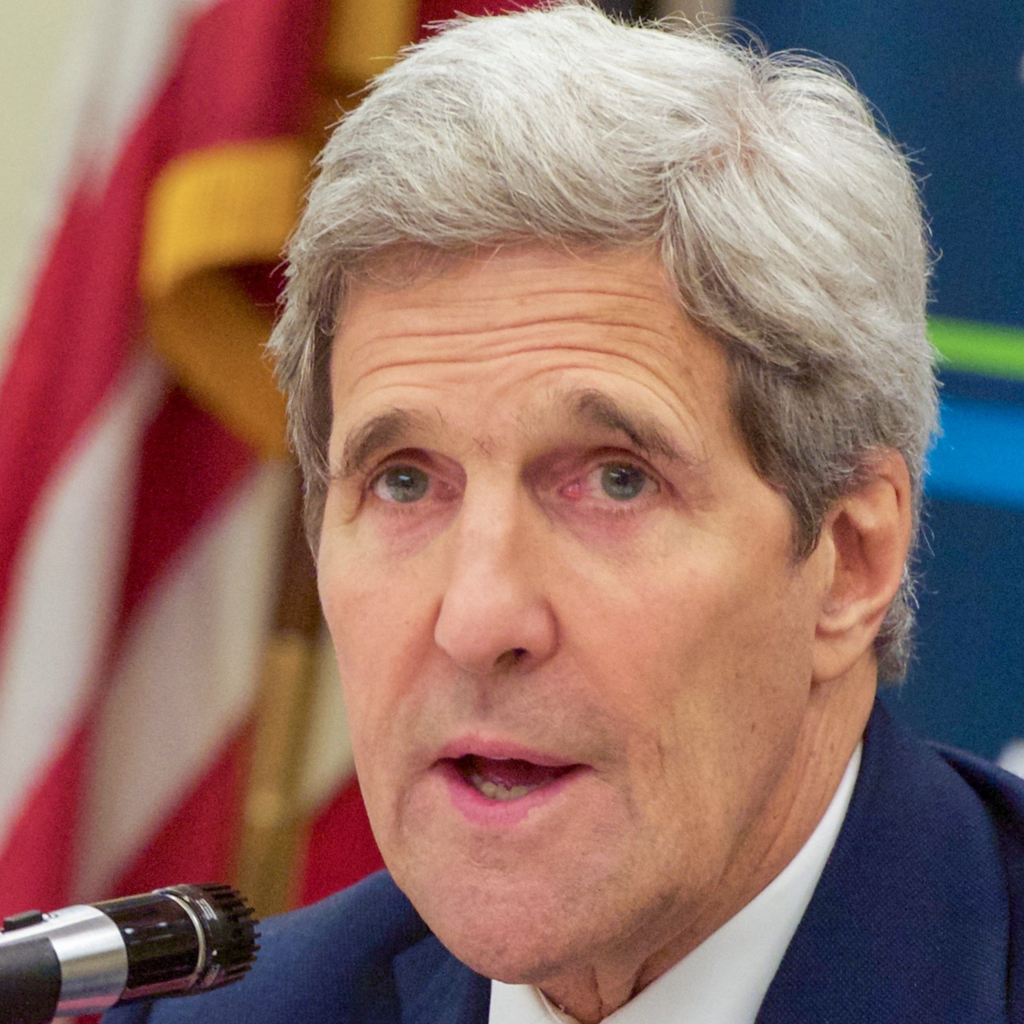
\includegraphics[width=0.32\linewidth]{./figures/00062.png}
      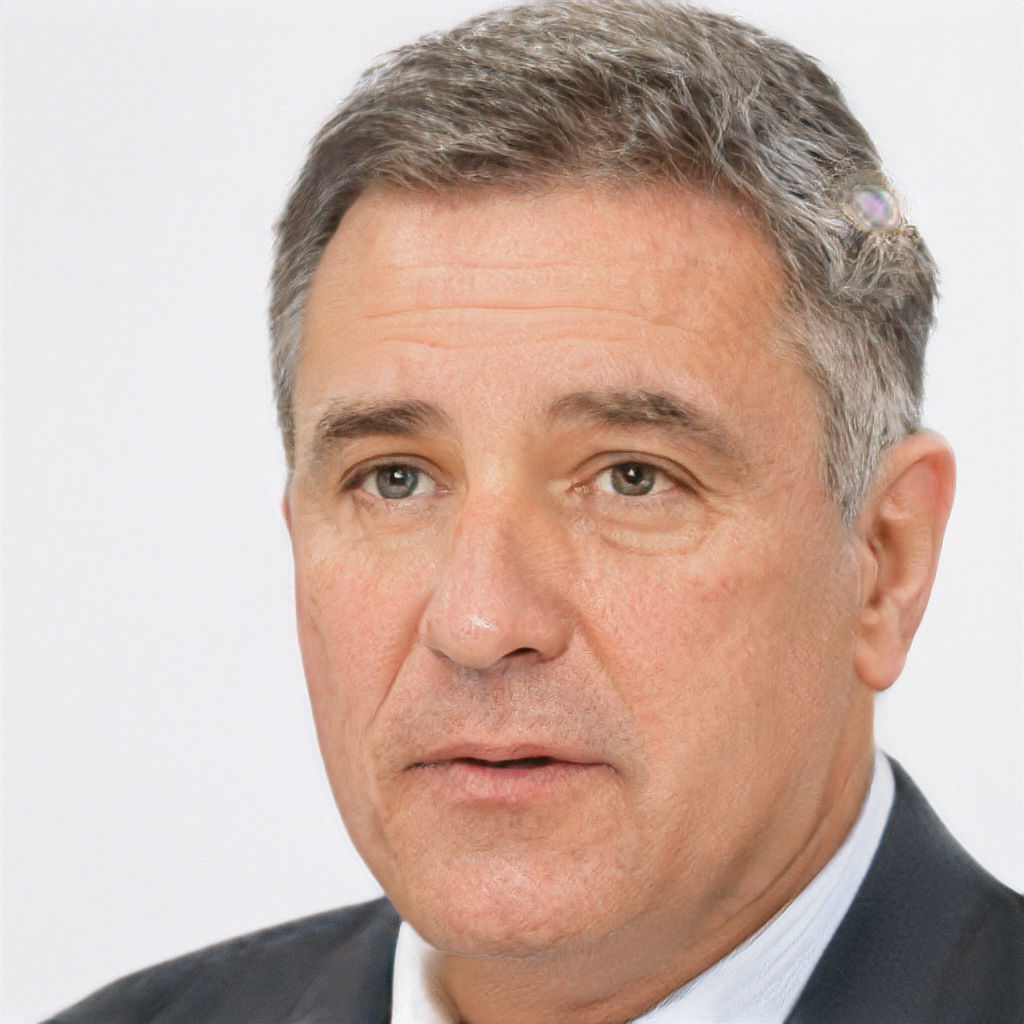
\includegraphics[width=0.32\linewidth]{./figures/style_gan_ffhq_example304.jpg}
      \end{figure}
    \end{frame}

    \begin{frame}{What blows the con?}
      \begin{figure}
        \includestandalone[width=0.32\linewidth]{./figures/fft_ffhq_val}
        \includestandalone[width=0.32\linewidth]{./figures/fft_gan_val}
        \includestandalone[width=0.32\linewidth]{./figures/fft_diff}
      \end{figure}
    \end{frame}

    \begin{frame}{Fake detectors}
      \begin{figure}
        \includestandalone[width=.49\linewidth]{./figures/classifier_plot}
        \includestandalone[width=.49\linewidth]{./figures/classifier_plot2}
      \end{figure}
      StyleGan-generated fakes can be classified with around 99\% accuracy this way \cite{frank2020leveraging}.
    \end{frame}

    \begin{frame}{Summary}
      \begin{itemize}
        \item For linearly separable binary problems weight inspection works great!
        \item Engineered features allow the inspection to reveal something about the data.
      \end{itemize}
    \end{frame}

    \section{Input Optimization}

    \begin{frame}{Motivation}
      Let's be honest. Most linearly separable binary problems are academic.
    \end{frame}

    \subsection{The problem with deep CNN}
    \begin{frame}{An input CNN-Layer}
      Kernel-shape: (3, 3, 1, 32)
      \begin{figure}
        \includestandalone{./figures/mnist_cnn}
        \caption{Plot of the input layer kernel weights trained on MNSIT.}
      \end{figure}
    \end{frame}

    \begin{frame}{Motivation Reloaded}
      \begin{itemize}
        \item How do we verify the correct operation of deep nonlinear networks?
        \item It is \textit{very} hard to interpret the weights of deep networks directly.
        \item Unit tests would require extensive re-training.
      \end{itemize}
    \end{frame}



    \begin{frame}{How to make a single neuron extremely happy}
      What if we turned the optimization problem around and optimized the input instead of the weights?
      Consider
      \begin{align}
        \max_\mathbf{x} y_i = f(\mathbf{x}, \theta) ,
      \end{align}
      with network weights $\theta$, input $\mathbf{x}$, and $y_i$, the activation of the $i$-th output neuron!
    \end{frame}

    \begin{frame}{The 6-neurons favorite input}
      Starting from $\mathbf{x} = \mathbf{1} \in \mathbb{R}^{1,28,28,1}$
      using image $\mu$-$\sigma$-normalization after every step
      with a step size of one and a positive update yields:
      \begin{figure}
        \includestandalone[width=0.6\linewidth]{./figures/grad_plot_mnist_6}
      \end{figure}
    \end{frame}

    \subsection{Saliency Maps and Integrated Gradients}

    \begin{frame}{The image net dataset}
      \begin{figure}
        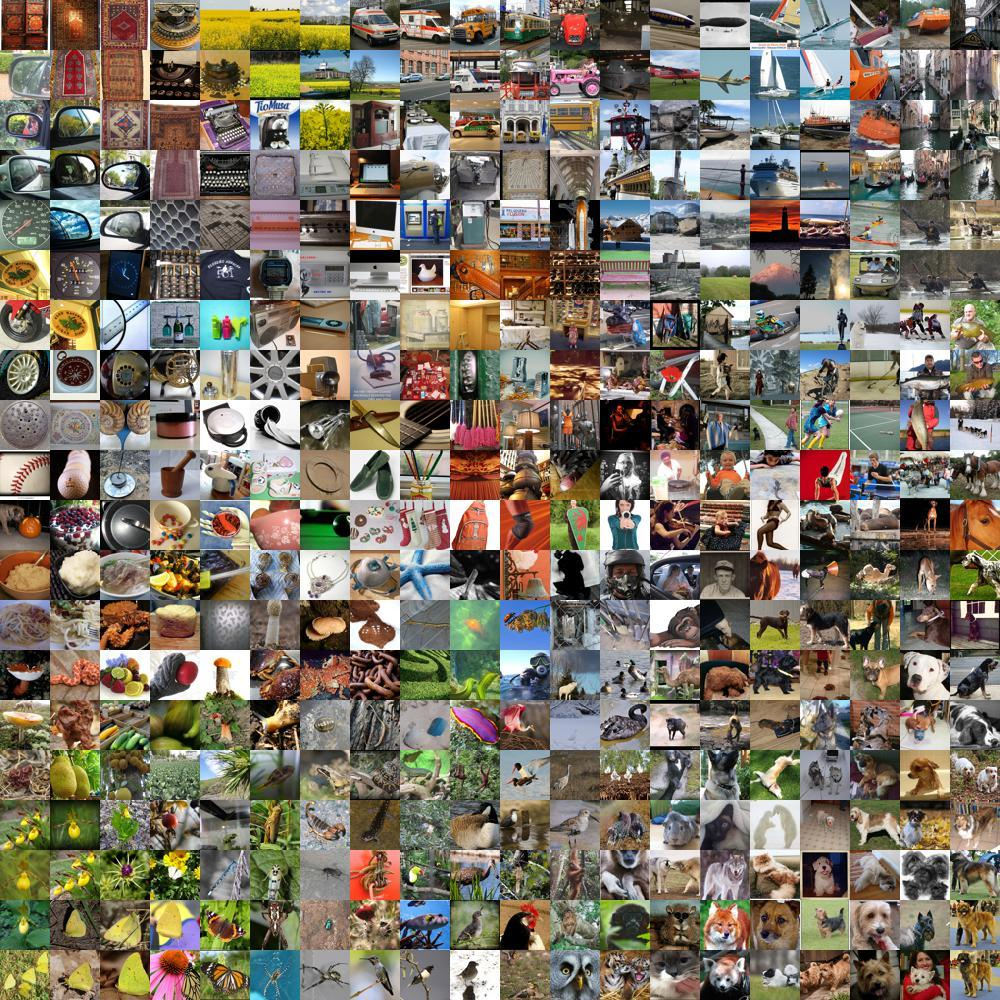
\includegraphics[width=0.6\linewidth]{figures/ImageNet.jpg}
        \caption{Image Net sample images as shown in \cite{russakovsky2015imagenet}. Today 14,197,122 annotated images. Typically with 1000 object
        categories.}
      \end{figure}
    \end{frame}

 
    \begin{frame}{AlexNet}
      \begin{figure}
        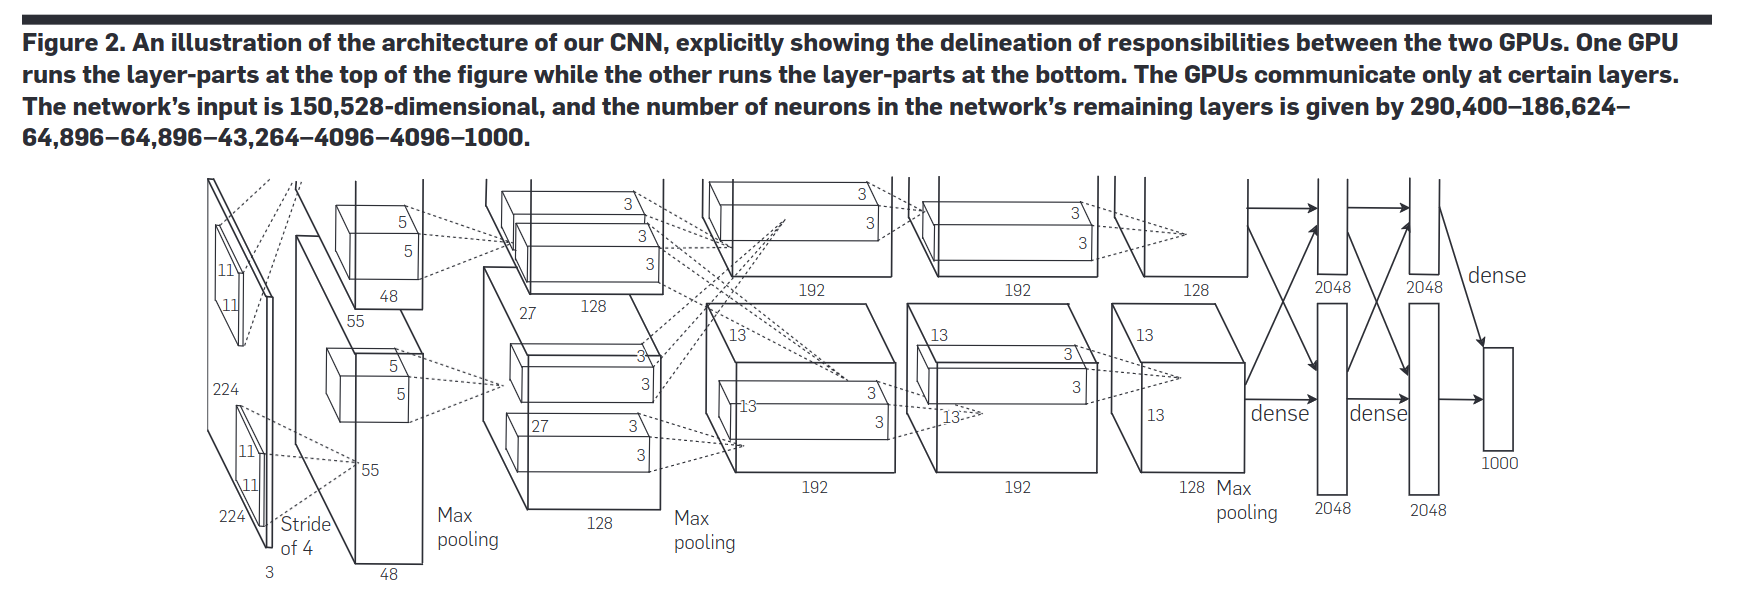
\includegraphics[width=\linewidth]{./figures/alexnet.png}
        \caption{The Alexnet-architecture used for classify imagenet in 2010  \cite{krizhevsky2017imagenet}}
      \end{figure}
    \end{frame}

    \begin{frame}{Early Alexnet layers}
      \begin{figure}
        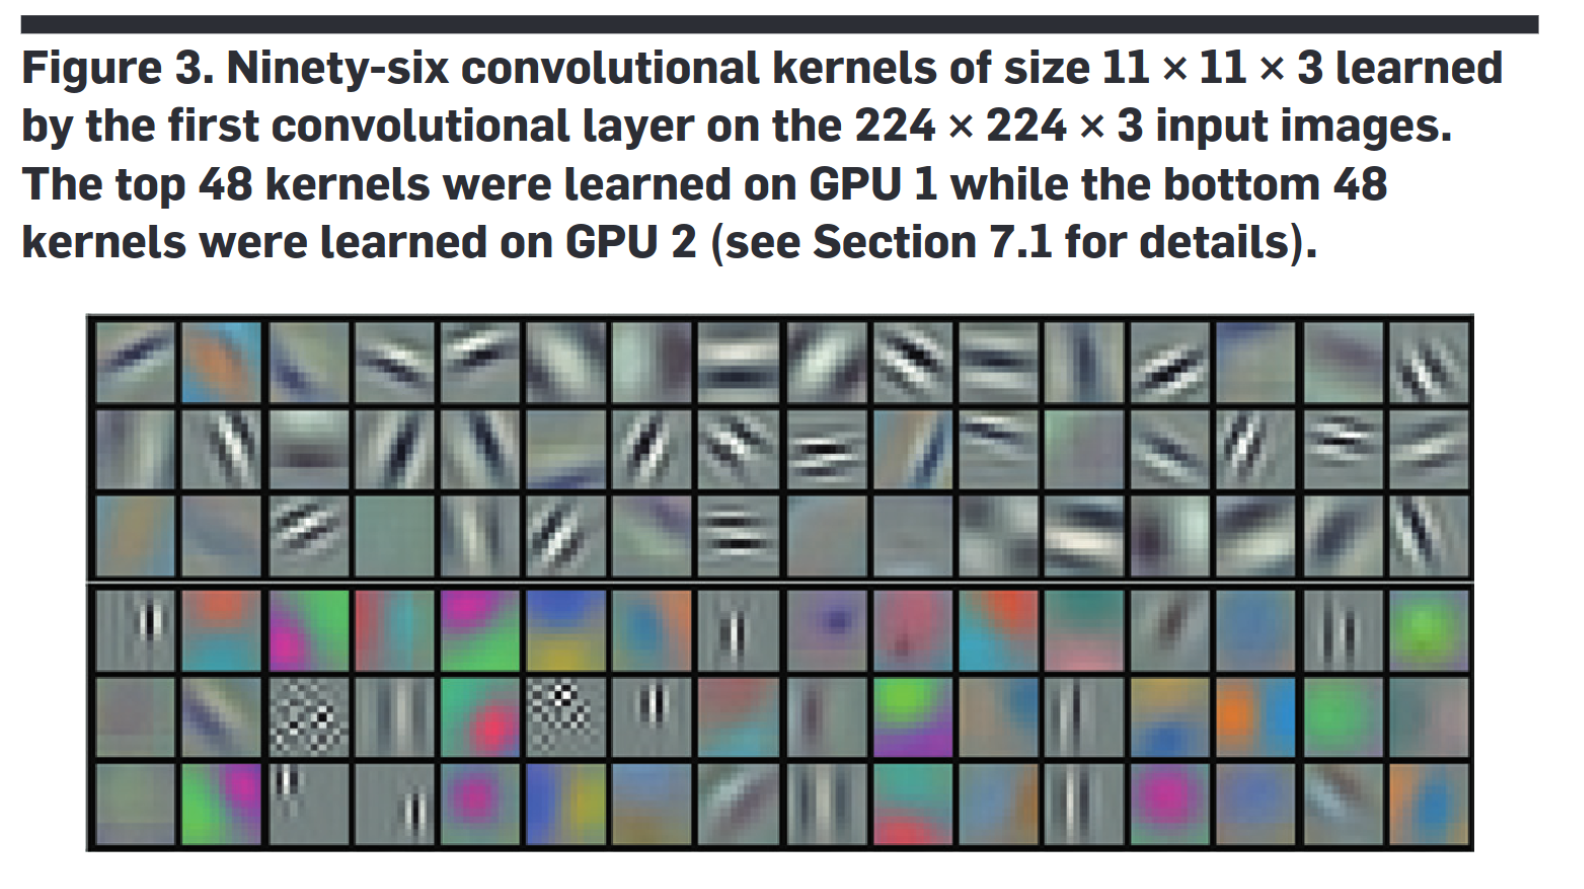
\includegraphics[width=0.9\linewidth]{./figures/alexnet_layer1.png}
        \caption{Plot from \cite{krizhevsky2017imagenet}.}
      \end{figure}
    \end{frame}

    \begin{frame}{Saliency Maps}
      \cite{simonyan2013deep} tell us to optimize
      \begin{align}
        \arg \max_{\mathbf{I}} S_c(\mathbf{I}) - \lambda | \mathbf{I} |_2^2 .
      \end{align}
      With $S_c$, the classification score for class c. $\mathbf{I}$ is the input image,
      and $|I|_2$ represents the 2-norm image channels. $\lambda$ is a regularization
      parameter.
    \end{frame}


    \begin{frame}{CNN-Saliency Map}
      \begin{figure}
      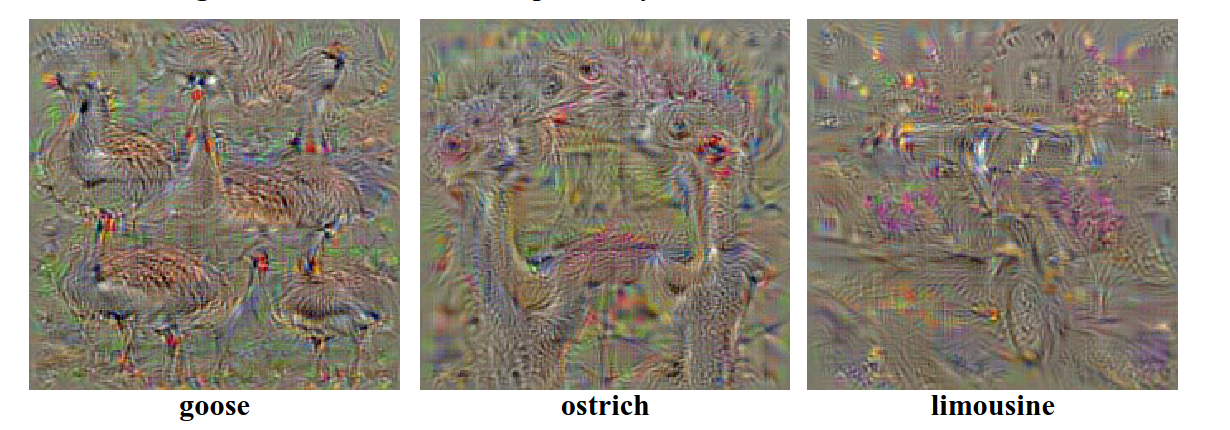
\includegraphics[width=0.9\linewidth]{./figures/sali.png}
      \caption{Input optimization saliency maps of a deep CNN trained on imagenet as shown in \cite{simonyan2013deep}.}
      \end{figure}
    \end{frame}

    \begin{frame}{Integrated-gradients}
    \cite{sundararajan2017axiomatic} propose to estimate individual input contributions
    to an output neuron via,
    \begin{align}
      \text{IntegratedGrads}_i(x) = (x_i - x_i') \cdot
      \sum_{k=1}^m \frac{\partial F (x' + \frac{k}{m} \cdot (x - x'))}{\partial x_i}. 
    \end{align}
    $\frac{\partial F}{\partial x_i}$ denotes the gradients with respect to the input color channels $i$.
    $\mathbf{x}'$ denotes a baseline black image. And $\mathbf{x}$ symbolizes an input we are interested in.
    Finally, $m$ denotes the number of summation steps from the black baseline image to the interesting input.
    \end{frame}


    \begin{frame}{Integrating the gradients of a multilayer CNN on MNIST}
      Integrated gradients for the zero neuron on the MNIST-validation set.
      \begin{figure}
      \includestandalone[width=0.49\linewidth]{./figures/ig_mnist_0}
      \end{figure}
    \end{frame}

    \begin{frame}{Images from the Wild}
      \begin{figure}
      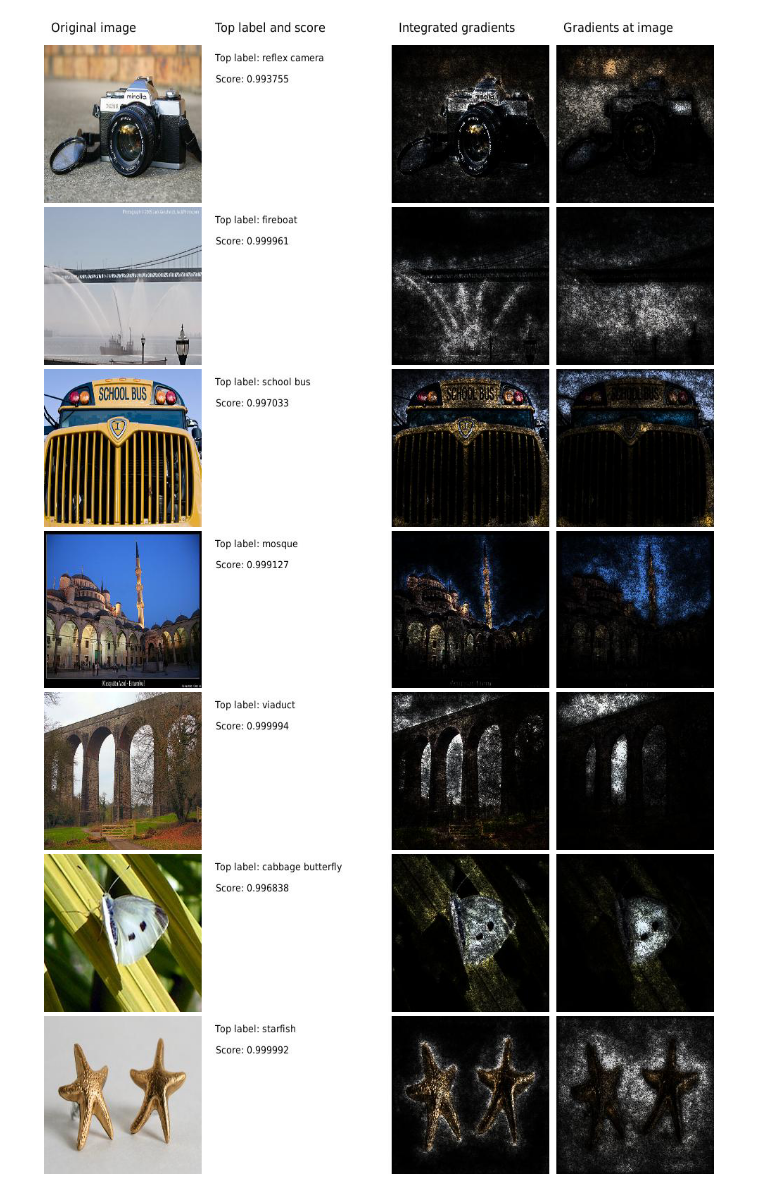
\includegraphics[scale=.16]{./figures/ig_paper.png}
      \caption{Integrated gradient visualization of input saliency for a very deep-CNN trained on Imagenet \cite{deng2009imagenet}.
      Image taken from \cite{sundararajan2017axiomatic}.}
      \end{figure}
    \end{frame}

    \begin{frame}{Conclusion}
      \begin{itemize}
        \item We can look at features and weights and work with input optimization to understand what is going on.
      \end{itemize}
    \end{frame}

    \section{Literature}
    \begin{frame}[allowframebreaks]{Literature}
      \printbibliography
    \end{frame}


\end{document}
